With the benchmark in place, we compare controller classes.
The right way to read this section is not as a leaderboard hunt, but as a boundary on what the benchmark actually supports.
The most stable ranking evidence comes from the within-domain repeatability runs, so we use those runs to define the paper's wording.

\begin{table*}[t]
\centering
\caption{Within-domain repeatability for the main-text controller set at the \(100\)-sample scale. Numbers are mean action regret, regret standard deviation, and mean compute-value calibration (Spearman \(\rho\)) over reruns. This table is intentionally used to constrain the paper's wording: it supports conditional ranking statements, but not a universal claim that one controller family wins everywhere.}
\label{tab:repeatability}
\begin{tabular}{llrrr}
\toprule
Domain & Controller & Mean regret & Std. regret & Mean calibration \\
\midrule
Arithmetic & \directpolicy & 0.119 & 0.027 & 0.604 \\
Arithmetic & \learnedoned & 0.122 & 0.033 & -0.566 \\
Arithmetic & \orderedscalar & 0.136 & 0.029 & 0.604 \\
Arithmetic & \triver exact-state & 0.140 & 0.019 & 0.713 \\
Arithmetic & \triver predicted-state & 0.323 & 0.052 & 0.221 \\
\midrule
Linear & \learnedoned & 0.062 & 0.020 & -0.611 \\
Linear & \directpolicy & 0.065 & 0.021 & 0.616 \\
Linear & \triver exact-state & 0.066 & 0.017 & 0.850 \\
Linear & \triver predicted-state & 0.126 & 0.026 & 0.300 \\
Linear & \orderedscalar & 0.145 & 0.046 & 0.684 \\
\bottomrule
\end{tabular}
\end{table*}

Table~\ref{tab:repeatability} tightens the claim boundary in two ways.
On linear equations, the robust statement is that \orderedscalar is consistently weakest, while \learnedoned, \directpolicy, and exact-state factorization form the stronger cluster.
On arithmetic, the larger-data repeatability runs show that \directpolicy and \learnedoned can outperform the simple scalar rule.
So the paper should argue for \emph{conditional scalar insufficiency}, not a universal theorem.

This repeatability table also sharpens the structured-controller story.
Exact-state factorization remains competitive in both domains and is strongest or near-strongest in the linear domain.
Predicted-state factorization, by contrast, remains substantially worse in both domains.
That exact-to-predicted separation is the main reason to interpret the structured-controller results as a deployment diagnosis rather than as evidence that structure is useless.

\paragraph{Deployment gap as the main structured-controller result.}
The most stable structured-controller result is not that \triver uniformly beats \directpolicy.
It does not.
Rather, the stable result is that exact-state and predicted-state performance are far apart.
This gap persists across regret, revision harm, and compute-value calibration.
That pattern makes it difficult to argue that the problem is only a missing value head or a missing post-hoc calibration rule.
The stronger interpretation is that state identification under noisy deployment is the bottleneck.
Target-cleaning and exact-state teacher-distillation probes in the appendix improve some domain/controller pairs, but they do not stack into a general rescue and they do not recover enough of the gap to overturn this reading.

\begin{figure}[t]
\centering
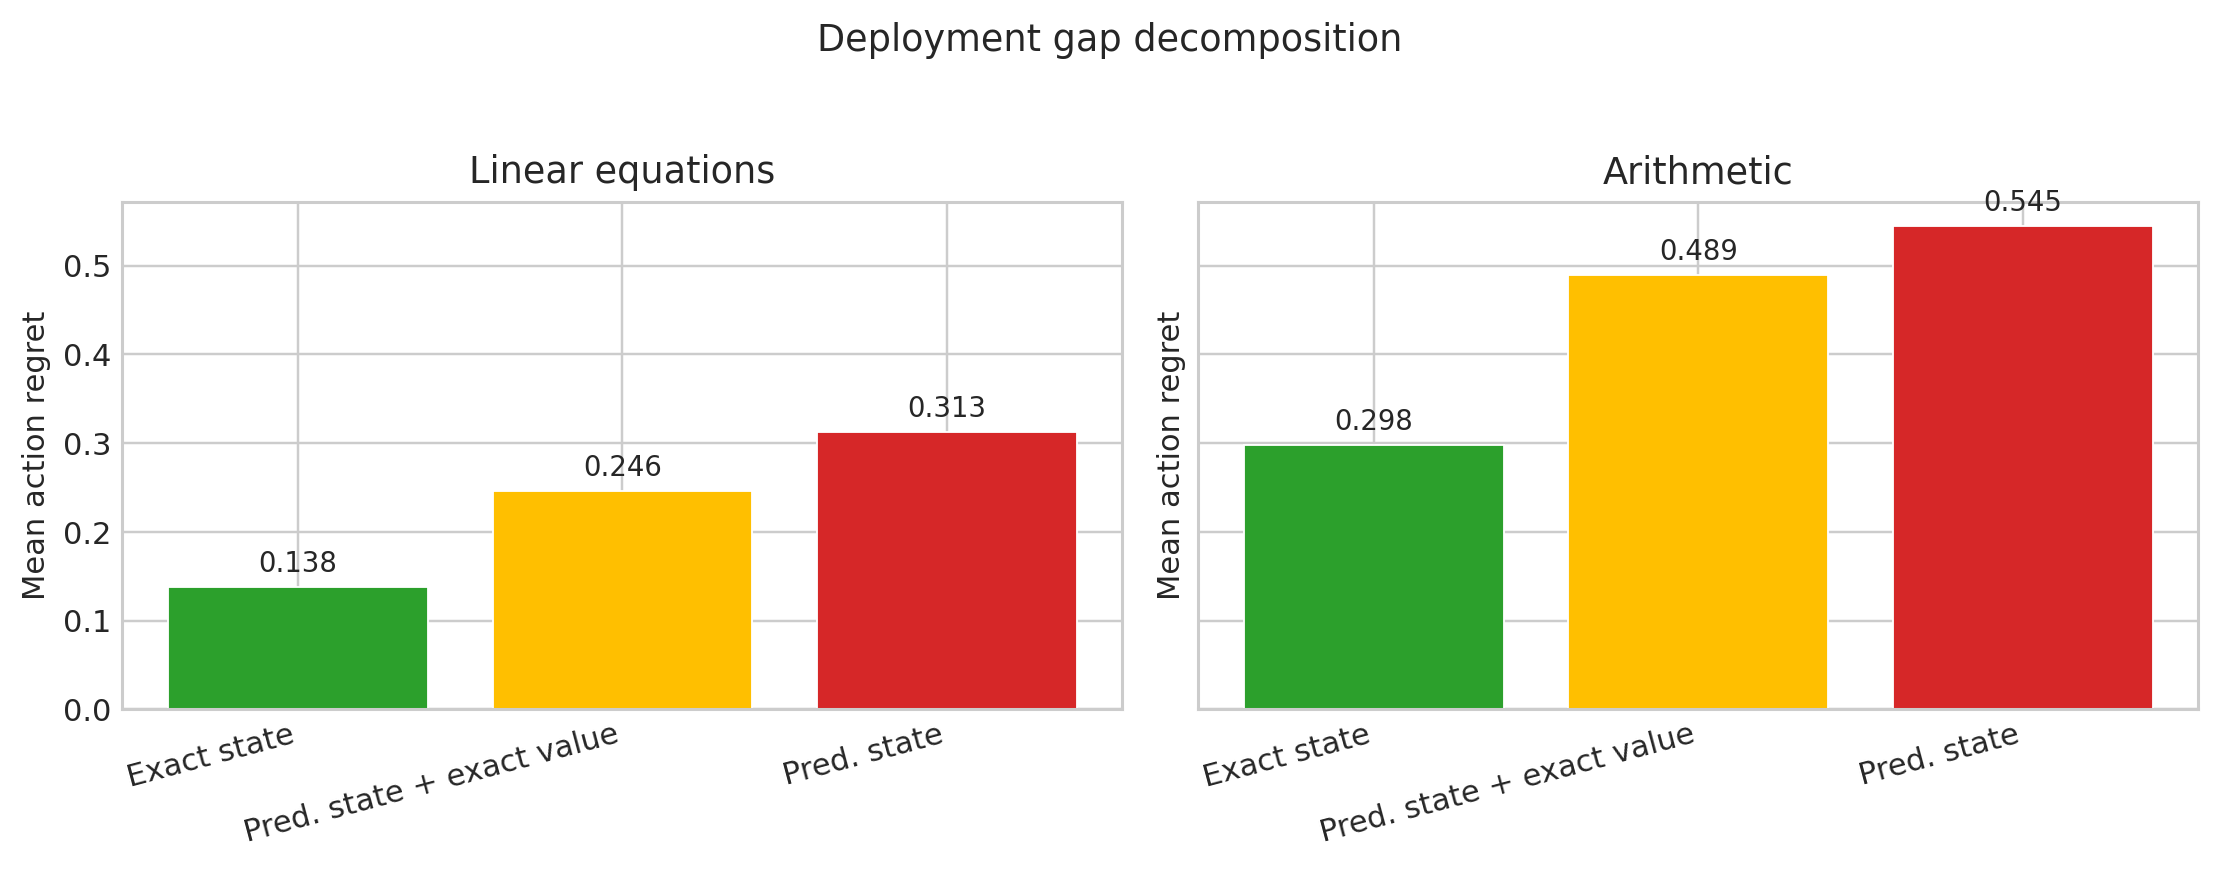
\includegraphics[width=\linewidth]{figures/deployment_gap.pdf}
\caption{Deployment-gap decomposition from matched factorized diagnostics. The exact-state row asks whether the structured controller contains useful signal in principle; the predicted-state row asks whether that signal survives deployment under learned state estimates. In both domains the exact-state controller is materially stronger, so the main failure mode is not ``structure is empty'' but ``state identification is too noisy at deployment time.''}
\label{fig:gap}
\end{figure}

Figure~\ref{fig:gap} makes this decomposition explicit.
The exact-state controller answers whether the factorization is meaningful at all.
The predicted-state controller answers whether the factorization survives deployment.
Our results imply that the answer to the first question is ``yes'' and the answer to the second is ``not reliably yet''.
That conclusion is strengthened rather than weakened by the appendix rescue probes: even the best domain-specific fixes remain well above the strongest learned one-dimensional baseline, so the paper should be read as a deployment diagnosis rather than an unfinished leaderboard chase.
